\documentclass[10pt,aspectratio=169,serif]{beamer}

\usepackage[fontset=none, scheme=plain]{ctex}
\IfFontExistsTF{Songti SC}{%
	\setCJKmainfont{Songti SC}[AutoFakeSlant=0.2]%
	\setCJKsansfont{Songti SC}[AutoFakeSlant=0.2]%
}{%
	\setCJKmainfont{FandolSong-Regular}[Extension=.otf,BoldFont=FandolSong-Bold,AutoFakeSlant=0.2]%
	\setCJKsansfont{FandolSong-Regular}[Extension=.otf,BoldFont=FandolSong-Bold]%
}
\usepackage{amsmath,amssymb,graphicx,tikz,booktabs,multicol,calligra}
\usepackage{pgfplots}
\pgfplotsset{compat=1.18}
\usepackage{tcolorbox}
\tcbuselibrary{skins}
\usepackage{XyygU}
\usepackage{caption}
\captionsetup[figure]{name=图,labelsep=period}

\usetikzlibrary{arrows.meta,positioning,calc}

\setlength{\abovedisplayskip}{0pt plus 2pt minus 2pt}
\setlength{\belowdisplayskip}{0pt plus 2pt minus 2pt}

\title[习题5.3]{习题 5.3　诱导公式}
\subtitle{复习巩固 \& 综合运用 \& 拓广探索}
\author{}
\institute{}
\date{2026-10-16}

\begin{document}

\begin{frame}
  \titlepage
\end{frame}

% ================= 复习巩固 =================
\begin{frame}[c]\Huge\centering 复习巩固\end{frame}

% ---------- 1 ----------
\begin{frame}[t]{复习巩固 1：求三角函数值}
\textbf{1.} 用诱导公式求下列三角函数值（可用计算工具，第(2)(3)(4)(5)题精确到 $0.0001$）：
\begin{enumerate}[(1)]
  \item $\cos\!\left(-\dfrac{17\pi}{4}\right)$； \qquad
  \item $\sin(-1574^\circ)$； \qquad
  \item $\sin(-2160^\circ52')$；
  \item $\cos(-1751^\circ36')$； \qquad
  \item $\cos 1615^\circ8'$； \qquad
  \item $\sin\!\left(-\dfrac{26\pi}{3}\right)$。
\end{enumerate}
\end{frame}

\begin{frame}[t]{复习巩固 1 解答}
\begin{tcolorbox}[colback=orange!10,colframe=orange,title=\textbf{解}]
先化到 $[0,2\pi)$（或 $[0,360^\circ)$），再用诱导公式。
\begin{enumerate}[(1)]
  \item $\cos\!\left(-\dfrac{17\pi}{4}\right)=\cos\!\left(4\pi+\dfrac{\pi}{4}\right)=\cos\dfrac{\pi}{4}=\alert{\dfrac{\sqrt2}{2}}$；
  \item $\sin(-1574^\circ)=-\sin(4\times360^\circ+134^\circ)=-\sin134^\circ=-\sin46^\circ\approx\alert{-0.7193}$；
  \item $\sin(-2160^\circ52')=-\sin(6\times360^\circ+0^\circ52')=-\sin0^\circ52'\approx\alert{-0.0151}$；
  \item $\cos(-1751^\circ36')=\cos(4\times360^\circ+311^\circ36')=\cos(360^\circ-48^\circ24')=\cos48^\circ24'\approx\alert{0.6639}$；
  \item $\cos1615^\circ8'=\cos(4\times360^\circ+175^\circ8')=\cos(180^\circ-4^\circ52')=-\cos4^\circ52'\approx\alert{-0.9964}$；
  \item $\sin\!\left(-\dfrac{26\pi}{3}\right)=-\sin\!\left(8\pi+\dfrac{2\pi}{3}\right)=-\sin\dfrac{2\pi}{3}=\alert{-\dfrac{\sqrt3}{2}}$。
\end{enumerate}
\end{tcolorbox}
\end{frame}

% ---------- 2 ----------
\begin{frame}[t]{复习巩固 2：求证}
\textbf{2.} 求证：
\begin{enumerate}[(1)]
  \item $\sin(360^\circ-\alpha)=-\sin\alpha$； \qquad
  \item $\cos(360^\circ-\alpha)=\cos\alpha$； \qquad
  \item $\tan(360^\circ-\alpha)=-\tan\alpha$。
\end{enumerate}
\end{frame}

\begin{frame}[t]{复习巩固 2 解答}
\begin{tcolorbox}[colback=orange!10,colframe=orange,title=\textbf{证明}]
利用“$360^\circ-\alpha$ 与 $-\alpha$ 终边相同”以及公式三：
\vspace{0.3em}
(1) $\sin(360^\circ-\alpha)=\sin(-\alpha)=\alert{-\sin\alpha}$；
\vspace{0.3em}
(2) $\cos(360^\circ-\alpha)=\cos(-\alpha)=\alert{\cos\alpha}$；
\vspace{0.3em}
(3) $\tan(360^\circ-\alpha)=\tan(-\alpha)=\alert{-\tan\alpha}$。
\vspace{0.3em}
\small（即“函数名不变，符号看 $360^\circ-\alpha$ 所在象限”，与公式四一致。）
\end{tcolorbox}
\end{frame}

% ---------- 3 ----------
\begin{frame}[t]{复习巩固 3：化简}
\textbf{3.} 化简：
\begin{enumerate}[(1)]
  \item $1+\sin(\alpha-2\pi)\sin(\pi+\alpha)-2\cos^2(-\alpha)$；
  \item $\sin(-1071^\circ)\sin99^\circ+\sin(-171^\circ)\sin(-261^\circ)$。
\end{enumerate}
\end{frame}

\begin{frame}[t]{复习巩固 3 解答}
\begin{tcolorbox}[colback=orange!10,colframe=orange,title=\textbf{解}]
(1) $\sin(\alpha-2\pi)=\sin\alpha$，$\sin(\pi+\alpha)=-\sin\alpha$，$\cos^2(-\alpha)=\cos^2\alpha$。
\[
\text{原式}=1+\sin\alpha(-\sin\alpha)-2\cos^2\alpha
=1-\sin^2\alpha-2\cos^2\alpha
=\cos^2\alpha-2\cos^2\alpha=\alert{-\cos^2\alpha}.
\]
(2) $\sin(-1071^\circ)=-\sin(3\times360^\circ-9^\circ)=-\sin(-9^\circ)=\sin9^\circ$；
$\sin99^\circ=\sin(90^\circ+9^\circ)=\cos9^\circ$；
$\sin(-171^\circ)=-\sin(180^\circ-9^\circ)=-\sin9^\circ$；
$\sin(-261^\circ)=-\sin(180^\circ+81^\circ)=\sin81^\circ=\cos9^\circ$。
\[
\text{原式}=\sin9^\circ\cos9^\circ+(-\sin9^\circ)\cos9^\circ=\alert{0}.
\]
\end{tcolorbox}
\end{frame}

% ---------- 4 ----------
\begin{frame}[t]{复习巩固 4：单位圆上的点}
\textbf{4.} 在单位圆中，已知角 $\alpha$ 的终边与单位圆的交点为 $P\!\left(-\dfrac35,\dfrac45\right)$，分别求角 $\pi+\alpha$，$-\alpha$，$\dfrac{\pi}{2}+\alpha$ 的正弦、余弦函数值。
\vspace{1em}
\begin{center}
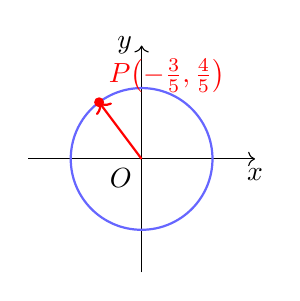
\begin{tikzpicture}[scale=0.9]
  \draw[->] (-1.6,0)--(1.6,0) node[below]{$x$};
  \draw[->] (0,-1.6)--(0,1.6) node[left]{$y$};
  \draw[thick,blue!60] (0,0) circle (1);
  \fill[red] (-0.6,0.8) circle (2pt);
  \draw[->,red,thick] (0,0)--(-0.6,0.8);
  \node[red,above right] at (-0.6,0.8) {$P\!\left(-\tfrac35,\tfrac45\right)$};
  \node[below left] at (0,0) {$O$};
\end{tikzpicture}
\end{center}
\end{frame}

\begin{frame}[t]{复习巩固 4 解答}
\begin{tcolorbox}[colback=orange!10,colframe=orange,title=\textbf{解}]
由 $P\!\left(-\dfrac35,\dfrac45\right)$ 在单位圆上，得
\[
\cos\alpha=-\frac35,\qquad \sin\alpha=\frac45.
\]
\vspace{0.3em}
\textbf{角 $\pi+\alpha$：}\quad $\sin(\pi+\alpha)=-\sin\alpha=\alert{-\dfrac45}$，\ $\cos(\pi+\alpha)=-\cos\alpha=\alert{\dfrac35}$。
\vspace{0.3em}
\textbf{角 $-\alpha$：}\quad $\sin(-\alpha)=-\sin\alpha=\alert{-\dfrac45}$，\ $\cos(-\alpha)=\cos\alpha=\alert{-\dfrac35}$。
\vspace{0.3em}
\textbf{角 $\dfrac{\pi}{2}+\alpha$：}\quad $\sin\!\left(\dfrac{\pi}{2}+\alpha\right)=\cos\alpha=\alert{-\dfrac35}$，\ $\cos\!\left(\dfrac{\pi}{2}+\alpha\right)=-\sin\alpha=\alert{-\dfrac45}$。
\end{tcolorbox}
\end{frame}

% ================= 综合运用 =================
\begin{frame}[c]\Huge\centering 综合运用\end{frame}

% ---------- 5 ----------
\begin{frame}[t]{综合运用 5：选择题}
\textbf{5.} 已知 $\sin\!\left(\dfrac{7\pi}{2}+\alpha\right)=\dfrac35$，那么 $\cos\alpha=$（\quad ）。

\vspace{1em}
\begin{columns}
\begin{column}{0.25\textwidth}
(A) $-\dfrac45$
\end{column}
\begin{column}{0.25\textwidth}
(B) $-\dfrac35$
\end{column}
\begin{column}{0.25\textwidth}
(C) $\dfrac35$
\end{column}
\begin{column}{0.25\textwidth}
(D) $\dfrac45$
\end{column}
\end{columns}
\end{frame}

\begin{frame}[t]{综合运用 5 解答}
\begin{tcolorbox}[colback=orange!10,colframe=orange,title=\textbf{解}]
\[
\sin\!\left(\frac{7\pi}{2}+\alpha\right)
=\sin\!\left(3\pi+\frac{\pi}{2}+\alpha\right)
=\sin\!\left(\pi+\frac{\pi}{2}+\alpha\right)
=-\sin\!\left(\frac{\pi}{2}+\alpha\right)
=-\cos\alpha.
\]
由 $-\cos\alpha=\dfrac35$，得 $\cos\alpha=-\dfrac35$。
\vspace{0.5em}
故选 \alert{(B)}。
\end{tcolorbox}
\end{frame}

% ---------- 6 ----------
\begin{frame}[t]{综合运用 6：已知条件求值}
\textbf{6.} 已知 $\sin(\pi+\alpha)=-\dfrac12$，计算：
\begin{enumerate}[(1)]
  \item $\sin(5\pi-\alpha)$； \qquad
  \item $\sin\!\left(\dfrac{\pi}{2}+\alpha\right)$； \qquad
  \item $\cos\!\left(\alpha-\dfrac{3\pi}{2}\right)$； \qquad
  \item $\tan\!\left(\dfrac{\pi}{2}-\alpha\right)$。
\end{enumerate}
\end{frame}

\begin{frame}[t]{综合运用 6 解答}
\begin{tcolorbox}[colback=orange!10,colframe=orange,title=\textbf{解}]
由 $\sin(\pi+\alpha)=-\sin\alpha=-\dfrac12$，得 $\sin\alpha=\dfrac12$，$|\cos\alpha|=\dfrac{\sqrt3}{2}$。
\vspace{0.3em}
(1) $\sin(5\pi-\alpha)=\sin(\pi-\alpha)=\sin\alpha=\alert{\dfrac12}$；
\vspace{0.3em}
(2) $\sin\!\left(\dfrac{\pi}{2}+\alpha\right)=\cos\alpha=\alert{\pm\dfrac{\sqrt3}{2}}$（象限未定，符号不确定）；
\vspace{0.3em}
(3) $\cos\!\left(\alpha-\dfrac{3\pi}{2}\right)=\cos\!\left(\dfrac{3\pi}{2}-\alpha\right)=-\sin\alpha=\alert{-\dfrac12}$；
\vspace{0.3em}
(4) $\tan\!\left(\dfrac{\pi}{2}-\alpha\right)=\cot\alpha=\dfrac{\cos\alpha}{\sin\alpha}=\alert{\pm\sqrt3}$。
\end{tcolorbox}
\end{frame}

% ---------- 7 ----------
\begin{frame}[t]{综合运用 7：三角形中的角}
\textbf{7.} 在 $\triangle ABC$ 中，试判断下列关系是否成立，并说明理由。
\begin{enumerate}[(1)]
  \item $\cos(A+B)=\cos C$； \qquad
  \item $\sin(A+B)=\sin C$；
  \item $\sin\dfrac{A+B}{2}=\sin\dfrac{C}{2}$； \qquad
  \item $\cos\dfrac{A+B}{2}=\cos\dfrac{C}{2}$。
\end{enumerate}
\end{frame}

\begin{frame}[t]{综合运用 7 解答}
\begin{tcolorbox}[colback=orange!10,colframe=orange,title=\textbf{解}]
在 $\triangle ABC$ 中 $A+B+C=\pi$，故 $A+B=\pi-C$，$\dfrac{A+B}{2}=\dfrac{\pi}{2}-\dfrac{C}{2}$。
\vspace{0.3em}
(1) $\cos(A+B)=\cos(\pi-C)=-\cos C$，与 $\cos C$ 一般不等，\alert{不成立}；
\vspace{0.3em}
(2) $\sin(A+B)=\sin(\pi-C)=\sin C$，\alert{成立}；
\vspace{0.3em}
(3) $\sin\dfrac{A+B}{2}=\sin\!\left(\dfrac{\pi}{2}-\dfrac{C}{2}\right)=\cos\dfrac{C}{2}$，与 $\sin\dfrac{C}{2}$ 一般不等，\alert{不成立}；
\vspace{0.3em}
(4) $\cos\dfrac{A+B}{2}=\cos\!\left(\dfrac{\pi}{2}-\dfrac{C}{2}\right)=\sin\dfrac{C}{2}$，与 $\cos\dfrac{C}{2}$ 一般不等，\alert{不成立}。
\end{tcolorbox}
\end{frame}

% ---------- 8 ----------
\begin{frame}[t]{综合运用 8：凑角求值}
\textbf{8.} 已知 $\sin\!\left(\dfrac{\pi}{3}-x\right)=\dfrac13$，且 $0<x<\dfrac{\pi}{2}$，求 $\sin\!\left(\dfrac{\pi}{6}+x\right)$ 和 $\cos\!\left(\dfrac{2\pi}{3}+x\right)$ 的值。
\end{frame}

\begin{frame}[t]{综合运用 8 解答}
\begin{tcolorbox}[colback=orange!10,colframe=orange,title=\textbf{解}]
注意到 $\left(\dfrac{\pi}{3}-x\right)+\left(\dfrac{\pi}{6}+x\right)=\dfrac{\pi}{2}$，
\[
\sin\!\left(\frac{\pi}{6}+x\right)
=\sin\!\left(\frac{\pi}{2}-\left(\frac{\pi}{3}-x\right)\right)
=\cos\!\left(\frac{\pi}{3}-x\right).
\]
由 $0<x<\dfrac{\pi}{2}$ 得 $-\dfrac{\pi}{6}<\dfrac{\pi}{3}-x<\dfrac{\pi}{3}$；又 $\sin\!\left(\dfrac{\pi}{3}-x\right)=\dfrac13>0$，故 $\dfrac{\pi}{3}-x\in\left(0,\dfrac{\pi}{3}\right)$，
\[
\cos\!\left(\frac{\pi}{3}-x\right)=\sqrt{1-\frac19}=\frac{2\sqrt2}{3}.
\]
所以 $\sin\!\left(\dfrac{\pi}{6}+x\right)=\alert{\dfrac{2\sqrt2}{3}}$。
\vspace{0.3em}
又 $\left(\dfrac{2\pi}{3}+x\right)+\left(\dfrac{\pi}{3}-x\right)=\pi$，
\[
\cos\!\left(\frac{2\pi}{3}+x\right)=\cos\!\left(\pi-\left(\frac{\pi}{3}-x\right)\right)=-\cos\!\left(\frac{\pi}{3}-x\right)=\alert{-\frac{2\sqrt2}{3}}.
\]
\end{tcolorbox}
\end{frame}

% ================= 拓广探索 =================
\begin{frame}[c]\Huge\centering 拓广探索\end{frame}

% ---------- 9 ----------
\begin{frame}[t]{拓广探索 9：含 $n$ 的化简}
\textbf{9.} 化简下列各式，其中 $n\in\mathbf Z$：
\begin{enumerate}[(1)]
  \item $\sin\!\left(\dfrac{n\pi}{2}+\alpha\right)$； \qquad
  \item $\cos\!\left(\dfrac{n\pi}{2}-\alpha\right)$。
\end{enumerate}
\end{frame}

\begin{frame}[t]{拓广探索 9 解答}
\begin{tcolorbox}[colback=orange!10,colframe=orange,title=\textbf{解：按 $n$ 被 $4$ 除的余数分类}]
(1)
\[
\sin\!\left(\frac{n\pi}{2}+\alpha\right)=
\begin{cases}
\sin\alpha, & n=4k,\\
\cos\alpha, & n=4k+1,\\
-\sin\alpha, & n=4k+2,\\
-\cos\alpha, & n=4k+3.
\end{cases}
\]
(2)
\[
\cos\!\left(\frac{n\pi}{2}-\alpha\right)=
\begin{cases}
\cos\alpha, & n=4k,\\
\sin\alpha, & n=4k+1,\\
-\cos\alpha, & n=4k+2,\\
-\sin\alpha, & n=4k+3.
\end{cases}\quad(k\in\mathbf Z)
\]
\end{tcolorbox}
\end{frame}

% ---------- 10 ----------
\begin{frame}[t]{拓广探索 10：单位圆的对称性}
\textbf{10.} 借助单位圆，还可以建立角的终边之间的哪些特殊位置关系？由此还能得到三角函数值之间的哪些恒等关系？
\end{frame}

\begin{frame}[t]{拓广探索 10 解答}
\begin{tcolorbox}[colback=orange!10,colframe=orange,title=\textbf{参考结论}]
\begin{itemize}
  \item \textbf{关于直线 $y=-x$ 对称：} 若两角终边关于 $y=-x$ 对称，则 $\beta=\dfrac{3\pi}{2}-\alpha$，于是
  \[
  \sin\!\left(\frac{3\pi}{2}-\alpha\right)=-\cos\alpha,\qquad
  \cos\!\left(\frac{3\pi}{2}-\alpha\right)=-\sin\alpha.
  \]
  \item \textbf{终边在同一直线上（反向）：} 即 $\beta=\pi+\alpha$，对应公式二；\textbf{关于 $x$ 轴、$y$ 轴、原点对称：} 分别对应公式三、公式四、公式二。
  \item \textbf{关于直线 $y=x$ 对称：} 即 $\beta=\dfrac{\pi}{2}-\alpha$，对应公式五。
\end{itemize}
\small 一般地，单位圆上点 $(x,y)$ 经反射/旋转后坐标的变化，都可化为三角函数间的恒等关系。
\end{tcolorbox}
\end{frame}

\begin{frame}[c]
  \begin{center}
    {\Huge\calligra Thanks!}
  \end{center}
\end{frame}

\end{document}
